\section{Prospective cases}
121 routine arrays were processed. The expected results are unknown but the number of calls is indicative of the number of calls required to be assessed during analysis.
\paragraph*{}
Using the Z score threshold of 2.374 there were a significant number of calls, with more than 1 in 3 cases having calls to investigate. A threshold of 3.55 resulted in a call in at least 1 in 9 arrays (Table \ref{tab:prospectivecasecalls}).
\paragraph*{}
The maximum number of calls in a single array is quite high, with one array having 199 calls at a threshold of 3.55.
\paragraph*{}
It is impossible to know if any of these are actually true positives.

\paragraph*{}
The average size of each call is just over three probes (Table \ref{tab:prosepectivecalls})
\begin{table}[h]
\centering
\caption[Prospective cases: The prevalence of calls]{Prospective Cases: The proportion of the 121 arrays where a call has been made, and the total number of calls made across a range of thresholds. At a threshold of 3.55 12\% of arrays contain a call. Across these 14 cases there are 246 calls, of which 119 is made in a single case.}
\label{tab:prospectivecasecalls}
\resizebox{\textwidth}{!}{%
\begin{tabular}{|l|l|l|}
\hline
Z score & \begin{tabular}[c]{@{}l@{}}\% of arrays with a call\\ (n)\end{tabular} & \begin{tabular}[c]{@{}l@{}}Total number of calls\\ (max calls in a single array)\end{tabular} \\ \hline
2.374   & 37 (45)                                                                           & 1760 (555)                                                                                   \\ \hline
3       & 16 (19)                                                                           & 591 (219)                                                                                    \\ \hline
3.55    & 12 (14)                                                                           & 246 (119)                                                                                    \\ \hline
3.75    & 12 (14)                                                                           & 186 (98)                                                                                     \\ \hline
4       & 10 (12)                                                                          & 125 (66)                                                                                     \\ \hline
4.25    & 7 (9)                                                                           & 90 (50)                                                                                      \\ \hline
\end{tabular}%
}
\end{table}
\newpage
\begin{figure}[h]
\centering
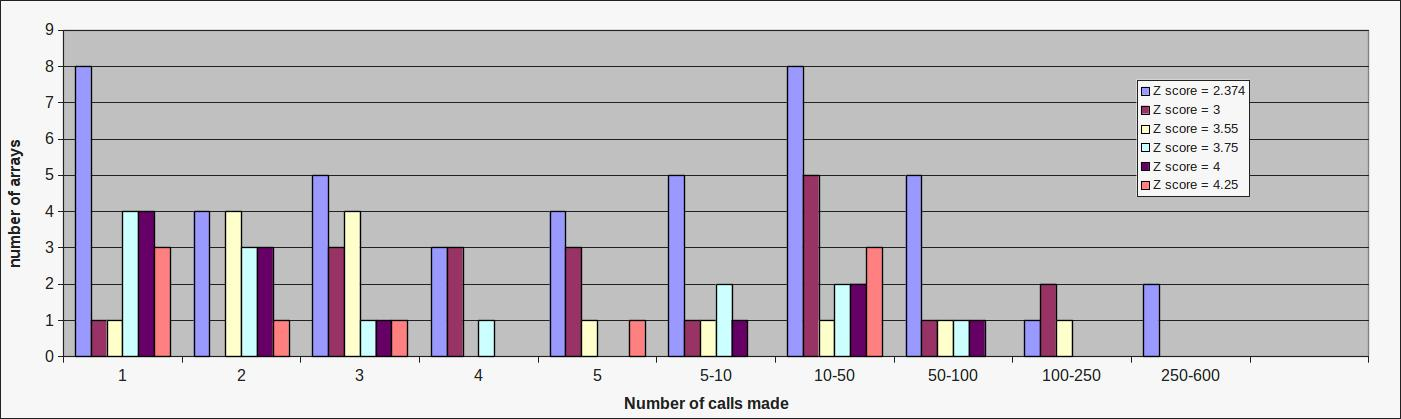
\includegraphics[width=1\linewidth]{./Figures/prospectivesamplecalls}
\caption{Prospective cases: The number of calls per array across a range of threshold in 121 prospective cases}
\label{fig:prospectivesamplecalls}
\end{figure}


\begin{table}[h]
\centering
\caption[Prospective cases: The number and size of calls]{Prospective cases: The average and maximum number of probes within a call during analysis of 121 prospective arrays.}
\label{tab:prosepectivecalls}
\resizebox{\textwidth}{!}{%
\begin{tabular}{@{}|l|l|l|l|@{}}
\hline
Z score & Average probes in call & Maximum probes in call & Number of calls \\ \hline
2.374   & 3.24                   & 8                      & 1760            \\ \hline
3       & 3.19                   & 7                      & 591             \\ \hline
3.55    & 3.14                   & 6                      & 246             \\ \hline
3.75    & 3.13                   & 6                      & 180             \\ \hline
4       & 3.1                    & 5                      & 125             \\ \hline
4.25    & 3.09                   & 5                      & 90              \\ \hline
\end{tabular}%
}
\end{table}

\section{Performance of SID}
When uploading a run of 96 arrays, initially each array is processed in approximately two minutes. However, due to the increasingly large features table, the time taken to process an array can increase to around 15 minutes.